\documentclass[oneside,a4paper,11pt,explicit]{book}
\usepackage[utf8]{inputenc}
\usepackage{icecream}
\usepackage[english]{babel}
\addto\captionsenglish{\renewcommand{\chaptername}{}}
\usepackage[accsupp]{axessibility}  % improves PDF readability for those with disabilities.
\usepackage[colorlinks = true,urlcolor  = blue,linkcolor = blue]{hyperref}
\usepackage{setspace}
\usepackage{listings}
\usepackage[most]{tcolorbox}
\usepackage{minitoc}


\renewcommand{\mtifont}{\large\sffamily}
\renewcommand{\mtcfont}{\small\sffamily}
\renewcommand{\mtcSfont}{\small\sffamily}
\renewcommand{\mtcSSfont}{\small\sffamily}
\renewcommand{\mtcSSSfont}{\small\sffamily}
\mtcsetpagenumbers{minitoc}{off} % turn off page numbering in minitocs
\addto{\captionsenglish}{% Making babel aware of special titles
	\renewcommand{\mtctitle}{Quick Links To Sections}
}
\setlength{\fboxrule}{5pt}
\setlength{\fboxsep}{4pt}

\definecolor{IceCreamLeaf}{HTML}{58743b}
\definecolor{IceCreamOrbit}{HTML}{732e00}
\definecolor{MACred}{rgb}{0.803921568627451, 0.3607843137254902, 0.3607843137254902}

\title{I.C.E.C.R.E.A.M. Tutorials}
\subtitle{\small Observing Earth from Above (Env 329) v24.06 \\
	\small Schmid College of Science and Technology, Chapman University}
\date{\today}

%% DOCUMENT
\setstretch{1.25}
\makeatletter
\begin{document}

\dominitoc

\faketableofcontents

\setcounter{chapter}{6} %Insert (Tutorial Number-1) Here; example for tutorial 4, enter 3

\chapter{Adding Elements To Maps} %Enter Tutorial Name Here

\vspace{-2em}

\minitoc

\hrule

\vspace{1em}

\begin{tcolorbox}[enhanced,frame style image=blueshade.png,
	opacityback=0.75,opacitybacktitle=0.25,
	colback=blue!5!white,colframe=blue!75!black,title={\Large \textbf{Objectives:}}]
	\large
	\begin{enumerate}
		\item Familiarize yourself with the basic map making features in QGIS.
		\item Practice creating a complete map of surface temperatures from Death Valley National Park that addresses our hypothesis. 
	\end{enumerate}
\end{tcolorbox}

\clearpage

%%%%%%%%%%%%%%%%%%%%%%%%%%%%%%%%%% Change Header to Have a Smaller Logo for Remainder of the Document
\fancyhead{}
\fancyhead[C]{\begin{tikzpicture}[overlay, remember picture]
		\fill[Blue2] (current page.north west) rectangle ($(current page.north east)+(0,-1in)$);
		\node[anchor=north west, text=white, font=\Large, minimum size=1in, inner xsep=5mm, align=left] at (current page.north west) {\bf{\MakeUppercase{\@title}}\\\@subtitle};
		\node[anchor=north east, minimum size=1in, inner xsep=5mm] at (current page.north east) {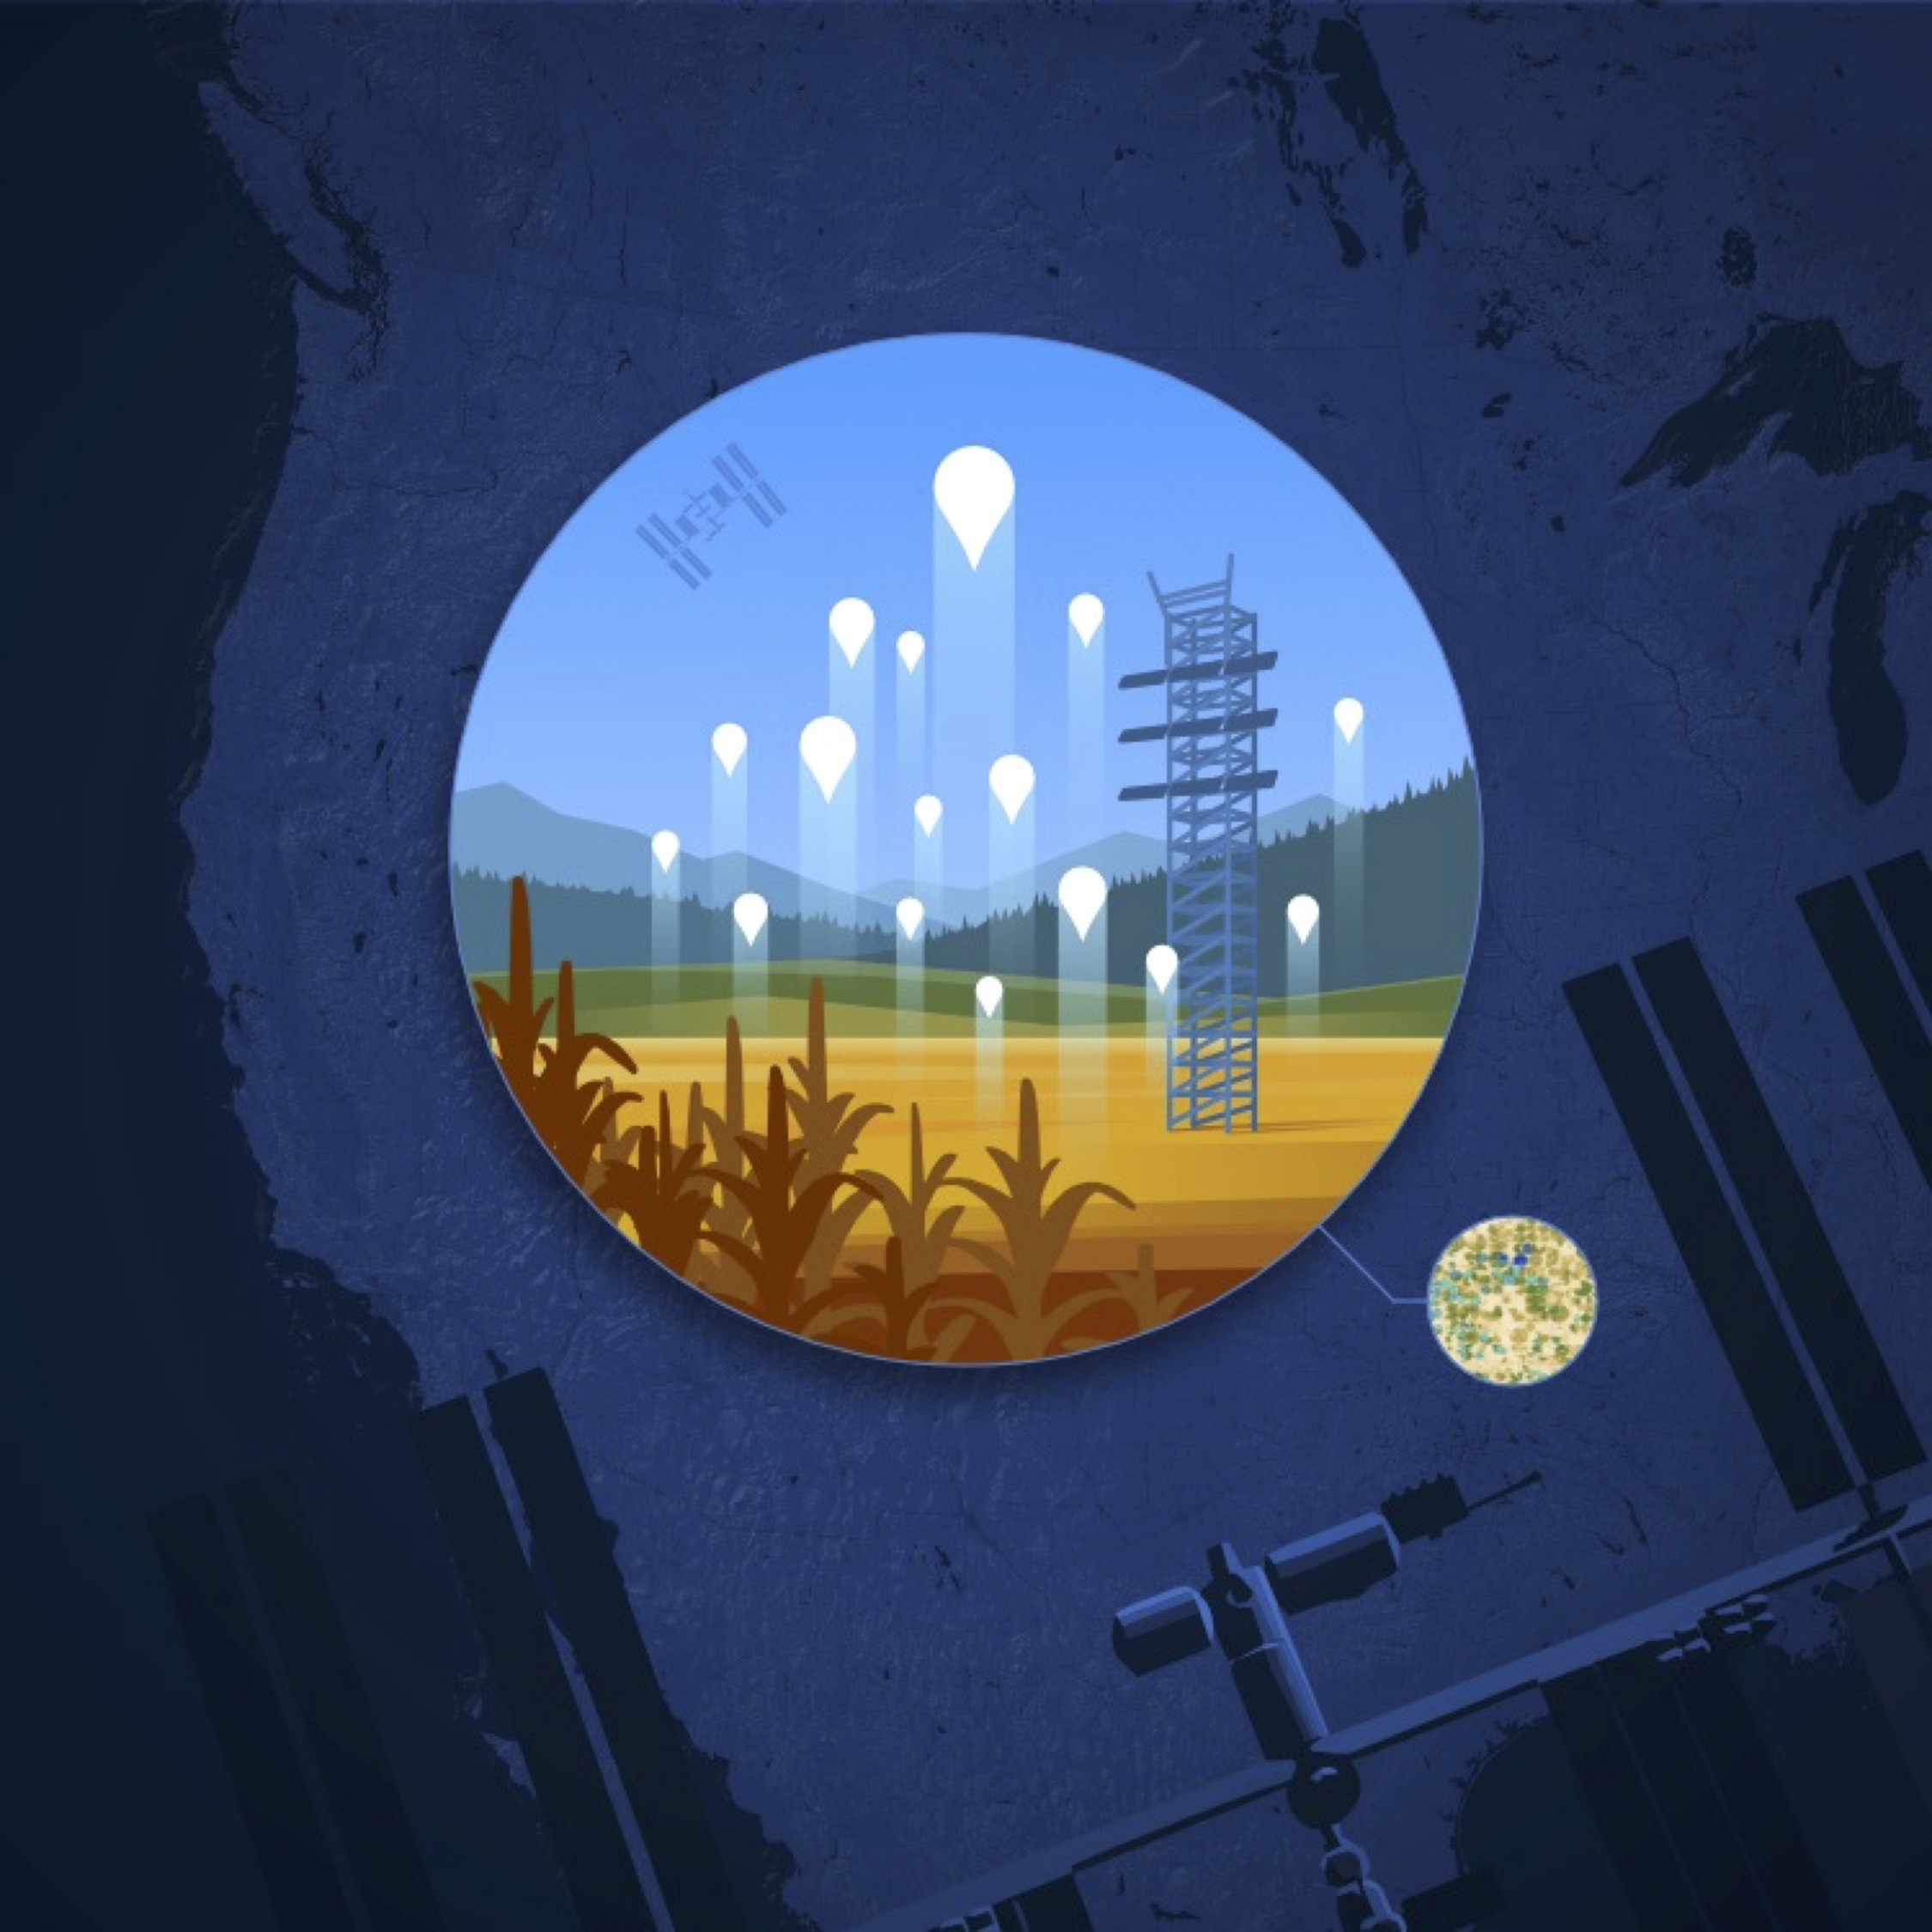
\includegraphics[scale=.03]{ECOSTRESS-BASE.jpg}};\end{tikzpicture}}
%%%%%%%%%%%%%%%%%%%%%%%%%%%%%%%%%%

\noindent\fbox{\begin{minipage}{.9665\textwidth}
			
	\vspace{1em}
	\begin{center}
		\textbf{\Large \underline{Motivation For Today's Tutorial: NASA Press Releases}}
	\end{center}
	
	\addcontentsline{toc}{section}{Motivation : NASA Press Releases}

	\vspace*{-1 em}
	
	\centerline{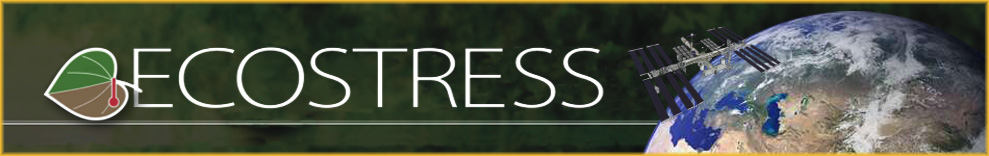
\includegraphics[width=\textwidth]{ecostress_banner.jpg}}

	We want to begin to use satellite remote sensing data to understand environmental events as they occur and use maps to effectively communicate those events to a broad audience. In \href{https://jeremydforsythe.github.io/icecream-tutorials/Tutorial4_AccessingRemoteSensingDataWithAppears/Tutorial4_AccessingRemoteSensingDataWithAppears.pdf}{Tutorial \#4: Accessing Remote Sensing Data With A$\rho\rho$EEARS} \& \href{https://jeremydforsythe.github.io/icecream-tutorials/Tutorial5_VisualizingDataWithQGIS/Tutorial5_VisualizingDataWithQGIS.pdf}{Tutorial \#5: Visualizing Data with QGIS}, we started to examine whether Death Valley broke its record of land surface temperature in July 2023. Today, our assignment is to create a map that will effectively communicate the answer. After you complete today's tutorial, you will have a basic working knowledge to create beautiful and informative maps. Later in the course, we will refine these skills to analyze current environmental events and make your maps available to newsmedia and other public-facing outlets. 
\end{minipage}}

\section{Data Wrangling}

\underline{If you have already completed \href{https://jeremydforsythe.github.io/icecream-tutorials/Tutorial5_VisualizingDataWithQGIS/Tutorial5_VisualizingDataWithQGIS.pdf}{Tutorial \#5: Visualizing Data with QGIS}:}

\vspace{.5em}

1a. Load the project file into QGIS that you saved in step \#9 by selecting the \textit{Project} menu, clicking \textit{Open} and navigating to where you saved the file. You should have a GIS environment loaded with the outline of Death Valley National Park from a vector shapefile and ECOSTRESS Land Surface Temperature from two GeoTIFF raster files resembling the image below:

\vspace{.5em}

\centerline{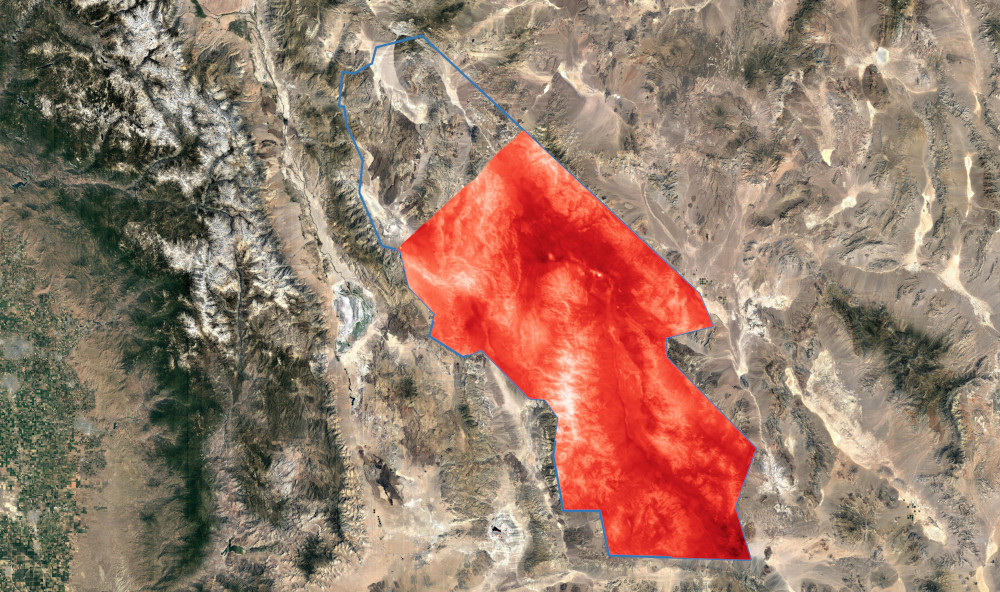
\includegraphics[width=\textwidth]{TempMap1.jpg}}

\vspace{.5em}

\underline{Or if you have \textbf{NOT} completed \href{https://jeremydforsythe.github.io/icecream-tutorials/Tutorial5_VisualizingDataWithQGIS/Tutorial5_VisualizingDataWithQGIS.pdf}{Tutorial \#5: Visualizing Data with QGIS}:}

\vspace{.5em} 

1b. Download the following datafiles, load them into a new QGIS project with a Google Satellite basemap, and adjust the colors and scales to match the image above (refer to \href{https://jeremydforsythe.github.io/icecream-tutorials/Tutorial4_AccessingRemoteSensingDataWithAppears/Tutorial4_AccessingRemoteSensingDataWithAppears.pdf}{Tutorial \#4: Accessing Remote Sensing Data With A$\rho\rho$EEARS} \& \href{https://jeremydforsythe.github.io/icecream-tutorials/Tutorial5_VisualizingDataWithQGIS/Tutorial5_VisualizingDataWithQGIS.pdf}{Tutorial \#5: Visualizing Data with QGIS} as needed):

\begin{tcolorbox}[colback=yellow!5!white,title=\textbf{Datafiles}]
	\addcontentsline{toc}{section}{Datafiles}
	\large
        Here is a copy of the vector shapefile for the border of Death Valley National Park:
        \begin{enumerate}
            \item \href{https://jeremydforsythe.github.io/icecream-tutorials/Tutorial4_AccessingRemoteSensingDataWithAppears/DeathValleyNationalPark.zip}{DeathValleyNationalPark.zip}
        \end{enumerate}
	Here are copies of the ECOSTRESS GeoTIFF files for Death Valley:
	\begin{enumerate}
		\item \href{https://jeremydforsythe.github.io/icecream-tutorials/Tutorial4_AccessingRemoteSensingDataWithAppears/ECO2LSTE.001_SDS_LST_doy2023209214149_aid0001.tif}{\small ECO2LSTE.001\textunderscore SDS\textunderscore LST\textunderscore doy2023209214149\textunderscore aid0001.tif}
		\item \href{https://jeremydforsythe.github.io/icecream-tutorials/Tutorial4_AccessingRemoteSensingDataWithAppears/ECO2LSTE.001_SDS_LST_doy2023209214057_aid0001.tif}{\small ECO2LSTE.001\textunderscore SDS\textunderscore LST\textunderscore doy2023209214057\textunderscore aid0001.tif}
	\end{enumerate}
\end{tcolorbox}

\section{Starting a Print Layout}

\begin{tcolorbox}[colback=yellow!5!white,colframe=IceCreamLeaf,title=\textbf{The \textit{Print Layout} Feature in QGIS}]
So you've got data visualized in the QGIS environment! You can interact with it by zooming/scrolling around the main window of QGIS or invite your closest friends over for a GIS viewing party on your laptop, but this isn't really a great map yet. The reason is that a GIS file is not an image. Rather, it saves the state of the GIS program, with references to all the data layers, their labels, colors, etc. So for someone who doesn’t have the data or the same QGIS program, the project file will be useless. 

\vspace{.5em}

You could export it as an image file as we did in \href{https://jeremydforsythe.github.io/icecream-tutorials/Tutorial5_VisualizingDataWithQGIS/Tutorial5_VisualizingDataWithQGIS.pdf}{Tutorial \#5: Visualizing Data with QGIS}, but that's just an image like the one we have on the bottom of page 2. If you were to give this to anyone on the streets of New York they would return a confused face to you as they struggled to understand any meaning of the image. They would ask questions like: ``What am I looking at here... where is this location?'', ``What does the red mean?'' \& ``Hey Boss... Why don't you get out of my way and lemme get on with ordering my bagel?'' Luckily, with QGIS you can create and export annotated maps to a format that anyone can read via the \href{https://docs.qgis.org/3.34/en/docs/training_manual/map_composer/map_composer.html}{\textit{Print Layout}} feature. The day is saved.

\centerline{\includegraphics[width=.25\textwidth]{Bagel.png}}

\vspace{-1em}

\end{tcolorbox}

\vspace{.5em}

2. To start a new print layout go to the \textit{Project} menu, then select \textit{New Print Layout}. Enter whatever name you wish (e.g., Death Valley Zoomed In).

\vspace{.5em}

\centerline{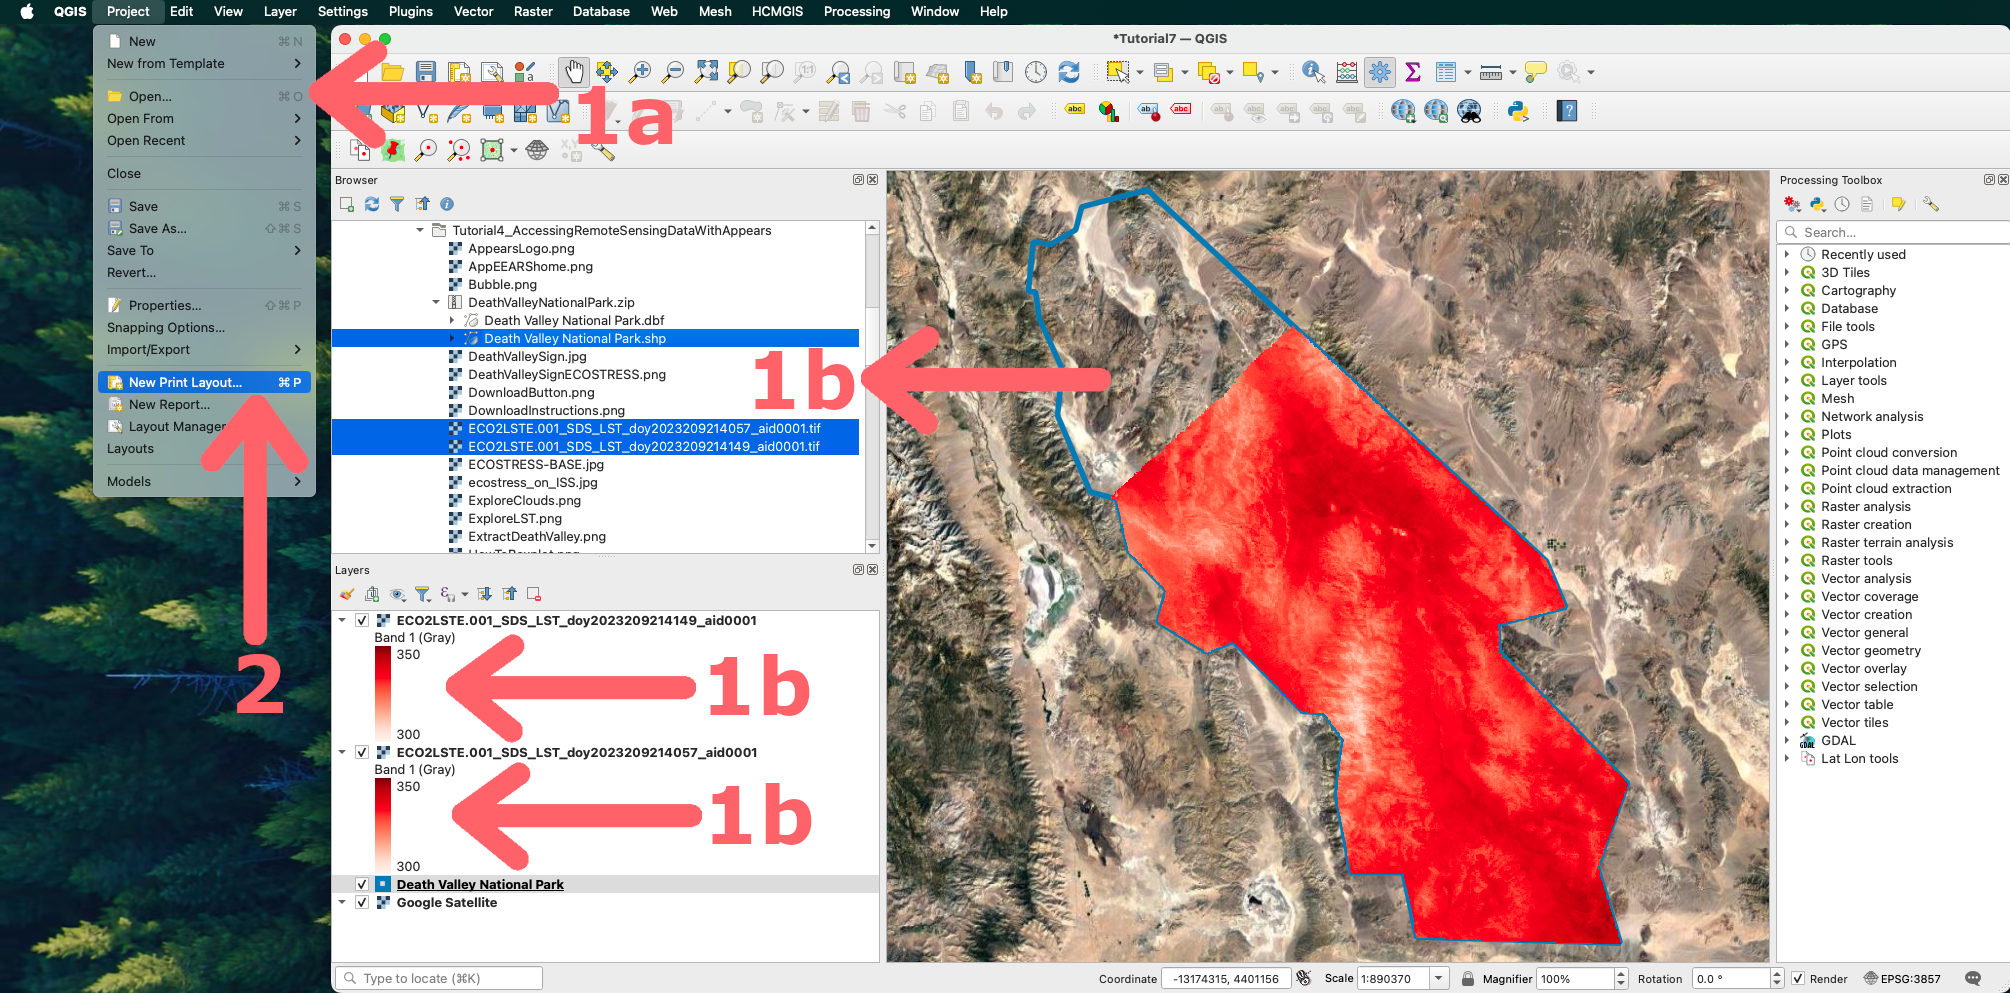
\includegraphics[width=\textwidth]{StartPrintLayout.png}}

3. Now, select the menu \textit{Add Item}, then \textit{Add Map}. Start at one corner of the white rectangle window and drag it to the opposite diagonal corner to set the map space. You will see that the rectangle window will be rendered with the map from the QGIS panel in the main window.

\kulbox{\textbf{NOTE:} You now have two QGIS windows open, what we refer to here as the main one is the QGIS window that you have been working with so far. It has the panel that displays your basemap, any data layers you have loaded in, the browser panel and the layers panel. The second window is the \textit{Print Layout} window that we are making our map in. The two windows communicate with each other. For instance, if you were to scroll and zoom around in the main panel of the QGIS window the map we just rendered in the \textit{Print Layout} window would update to that view, unless we lock it in the Item window. More on this ahead...}

4. Click on the \textit{Item Properties} tab.

\vspace{.5em}

\centerline{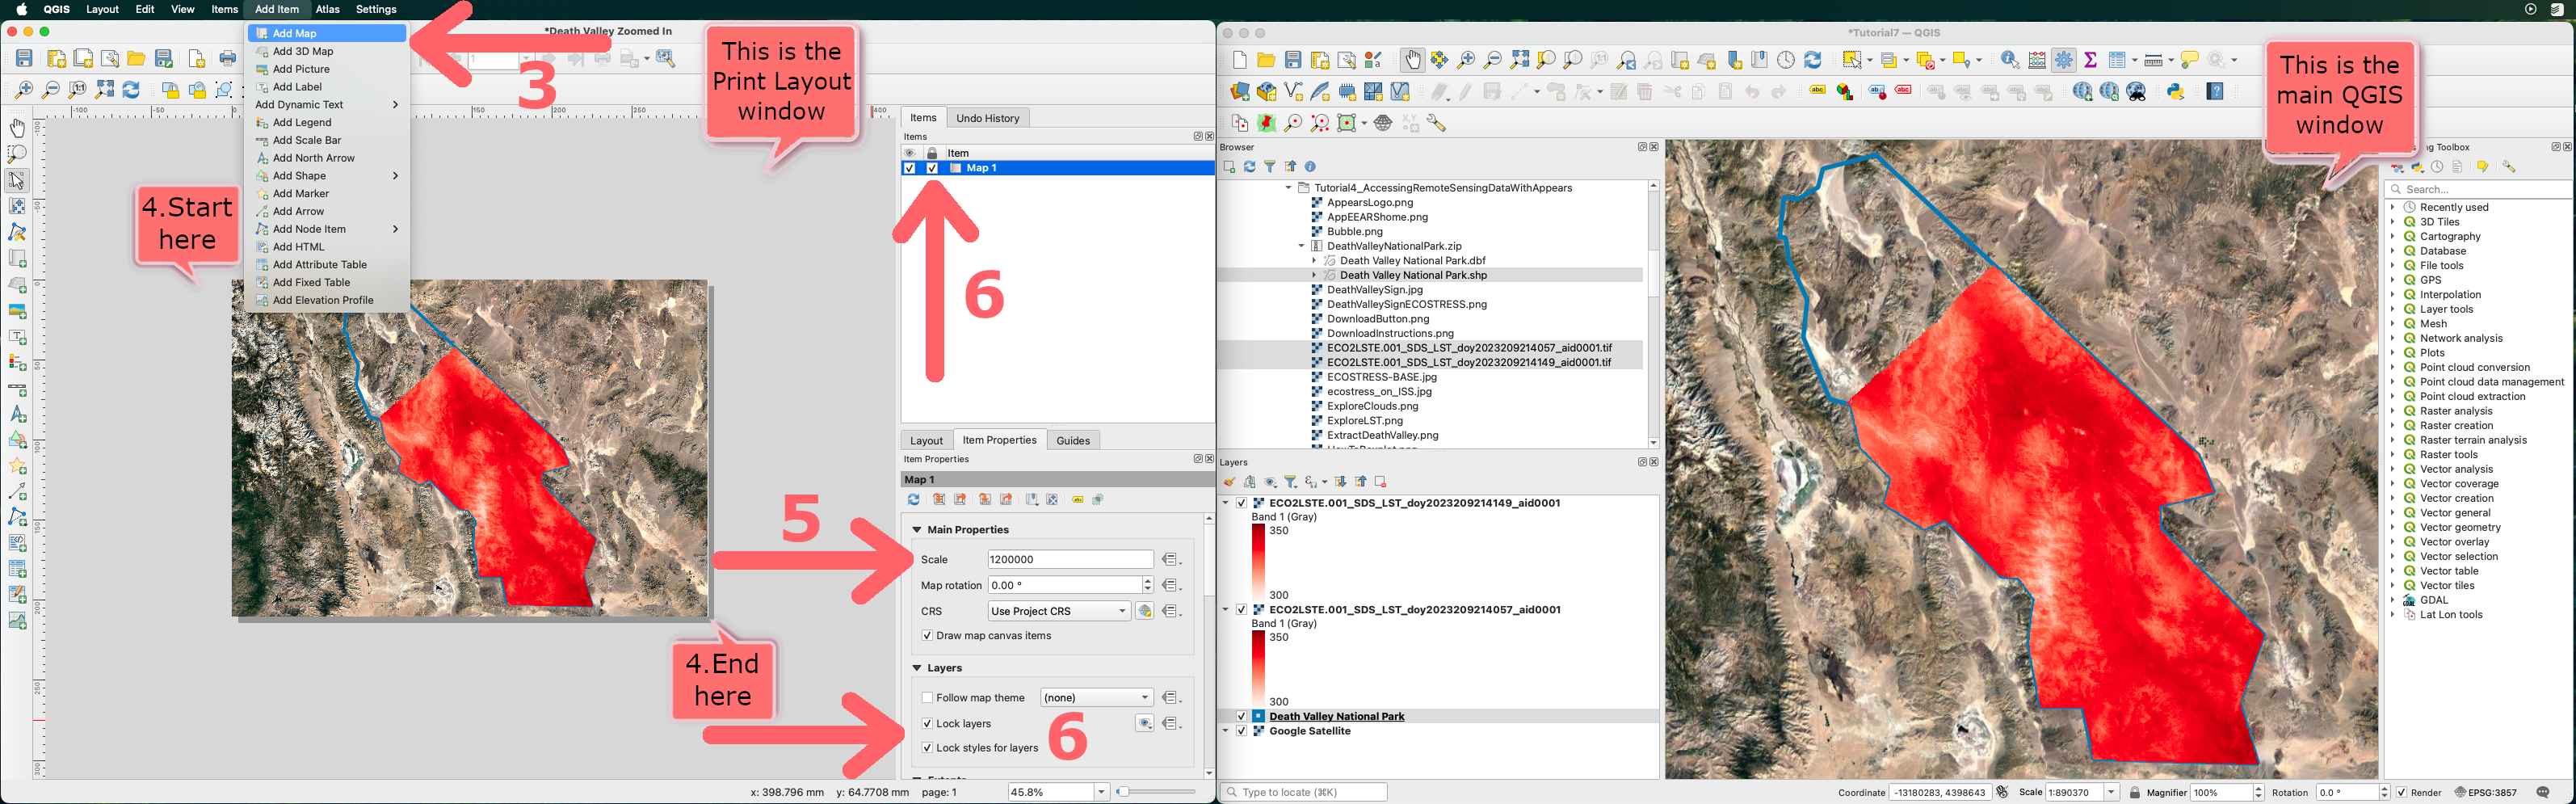
\includegraphics[width=\textwidth]{AddMapToPrintLayout.png}}


5. Adjust the \textit{Scale}, which is the zoom level, to 1200000 and press Enter. Determining a zoom level is a matter of trial and error based on what features of the map you wish to represent. 

6. Check the \textit{Lock layers} box, \textit{Lock layer styles} box, and lock icon box next to the layer of our map. As mentioned in the earlier note box, this will ensure that if we turn off some layers, pan or zoom, or change the symbology of any of the layers in the main QGIS window, our view here in the \textit{Print Layout} will not change.

\section{Basic Map Elements}

\centerline{\includegraphics[width=\textwidth]{AddLegend.png}}

\subsection{Adding a Legend}

A legend's function is to describe the visual information contained in a map by explaining what the symbols and colors displayed on the map mean.

\vspace{.5em}

7. Select \textit{Map 1} from the \textit{Items} window.

8. From the \textit{Add Item} menu bar at the top, select \textit{Legend}. Draw the legend by clicking and dragging a box in a suitable place on the map. We selected the bottom-left corner. We can adjust its size and position later, so don't worry too much about how it looks right now.

9. Under \textit{Item Properties} enter ``Land surface temperature ($^{\circ}$ F)'' as a title.

10. For \textit{Wrap text on} enter an underscore ``\_''. This will split the title of your legend into two lines at the underscore. 

11. Deselect the check box next to \textit{Auto update} to allow us to further customize what is displayed in the legend. Otherwise, QGIS would automatically update the legend with all the data layers we have loaded back on the other main window, including the basemap.

12. We matched the temperature ranges for both layers, so only one legend entry is necessary. Remove all legend entries, except one of our ECOSTRESS surface temperature layers, by selecting the ones you want to remove and using the minus button. 

\vspace{.5em}

The SI unit of temperature set for the International System of Units is Kelvin (K), which is how the land surface temperature observations made by ECOSTRESS are reported. You can use the formulas below to convert K into Celsius or Fahrenheit, which are generally more widely known by your target audiences. 
\begin{itemize}
	\item $C = K - 273.15$
	\item $F = (K - 273.15) \cdot \frac{9}{5} + 32$
\end{itemize}

13. To change the scale of the legend bar, double click on the scale in the \textit{Legend Items} property window.

\vspace{.25em}

\centerline{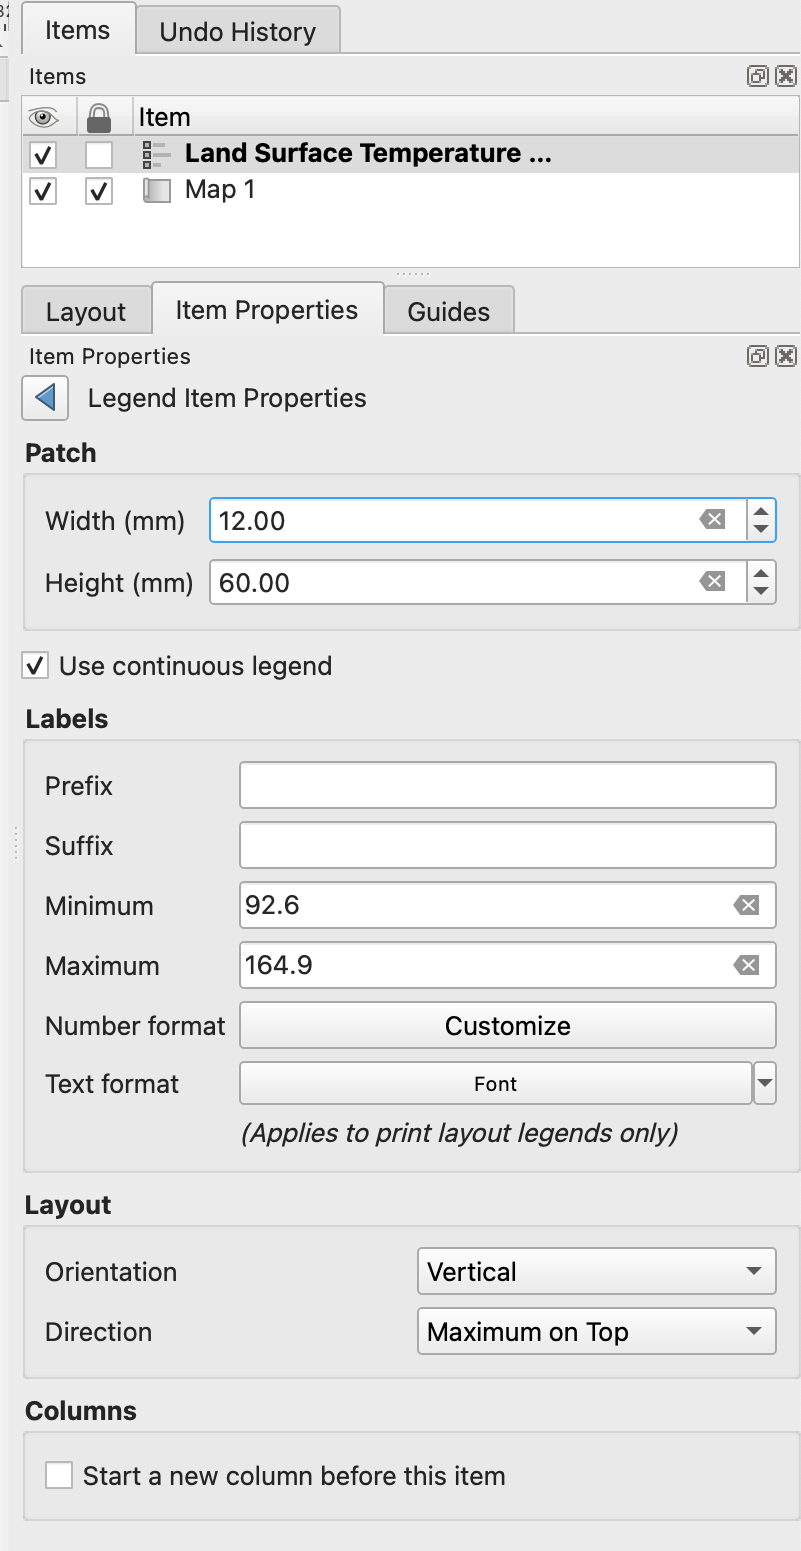
\includegraphics[width=.5\textwidth]{tempscale.png}}

14. After converting to $^{\circ}$F, our land surface temperature yields a range of 92.6 to 164.9 $^{\circ}$F. Enter these values in place of the default minimum and maximum values. Let's also adjust the width of the legend to 12 mm and the height to 60 mm, or to your preferred size to ensure that you can see the color bar. When you have finished adjusting, use the back arrow to return to \textit{Legend Item Properties}.

15. Our legend labels are a little haphazard, since QGIS automatically creates them from the filenames we import. To adjust, double click on the ECO2LSTE.001SDSLSTdoy... label in the \textit{Legend Items} list. Instead, enter some useful information, perhaps the month ``July 2023''. 

16. QGIS has included band information, which is useful for rasters with multiple bands. Since ours only has one, double-click on ``Band 1 (Gray)'' and make it blank by replacing the label with a spacebar press.

\kulbox{\centerline{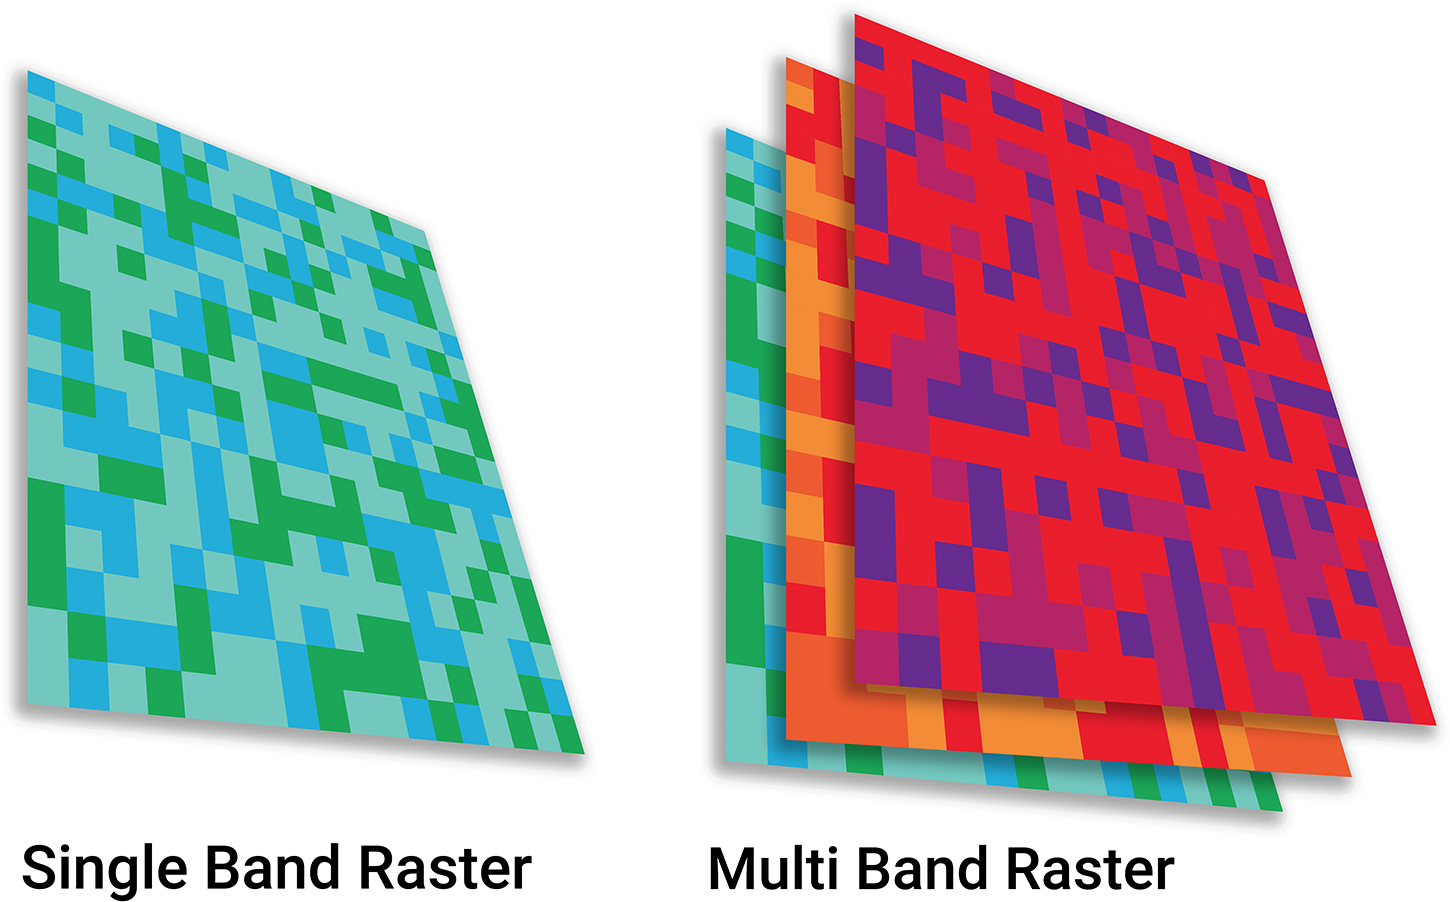
\includegraphics[width=.6\textwidth]{RasterBands.png}}

\vspace{.5em}

\textbf{NOTE:} Our rasters have a single band of data (measure of a single characteristic such as land surface temperature for one pass of ECOSTRESS). Other data sources often have multiple bands, representing data at the same spatial locations that vary along some other variable (such as time, or variable of interest). Basically, a band is represented by a single matrix of cell values, and a raster with multiple bands contains multiple spatially coincident matrices of cell values representing the same spatial area.} 

17. Let's make the legend look a little more professional by adjusting the background color. Scroll down in the \textit{Legend Item Properties} list and look for the \textit{Background} section. Use the arrow to expand your options. Here you can change the color, but for now let's leave it white. Instead, adjust the \textit{Opacity} to 75\%. This makes the legend background more transparent, giving it a cleaner, more modern look. Finally, click and hold to adjust the position of the legend after all that editing. It should resemble the screenshot below.

\centerline{\includegraphics[width=\textwidth]{AdjustLegend.png}}

Let's add a couple more small details to bring this map to the next level.

\subsection{Adding a Scalebar}

It is important for the reader to know the scale of the maps, particularly when we are zoomed in this far. This is achieved with scalebars that can automatically be drawn by QGIS. 

\centerline{\includegraphics[width=\textwidth]{AddScalebar.png}}

18. With the map (likely named ``Map 1'' unless you changed it) highlighted in the \textit{Items} browser, click the \textit{Add Item} menu at the top of the screen and select \textit{Add Scalebar}.

19. Draw the scalebar on the main map in a logical place. Look for a place where you will not obscure any of the key information conveyed by the map. We picked the bottom right corner.

20. Under \textit{Item Properties}, you could adjust the style or units to your liking. We will leave it in km, but since the text is a little hard to read we will add a buffer. In the \textit{Scalebar Item Properties} scroll down until you see the ``Display'' section. Expand it using the arrow on its left and click inside the ``Font'' box:

\vspace{.25em}

\centerline{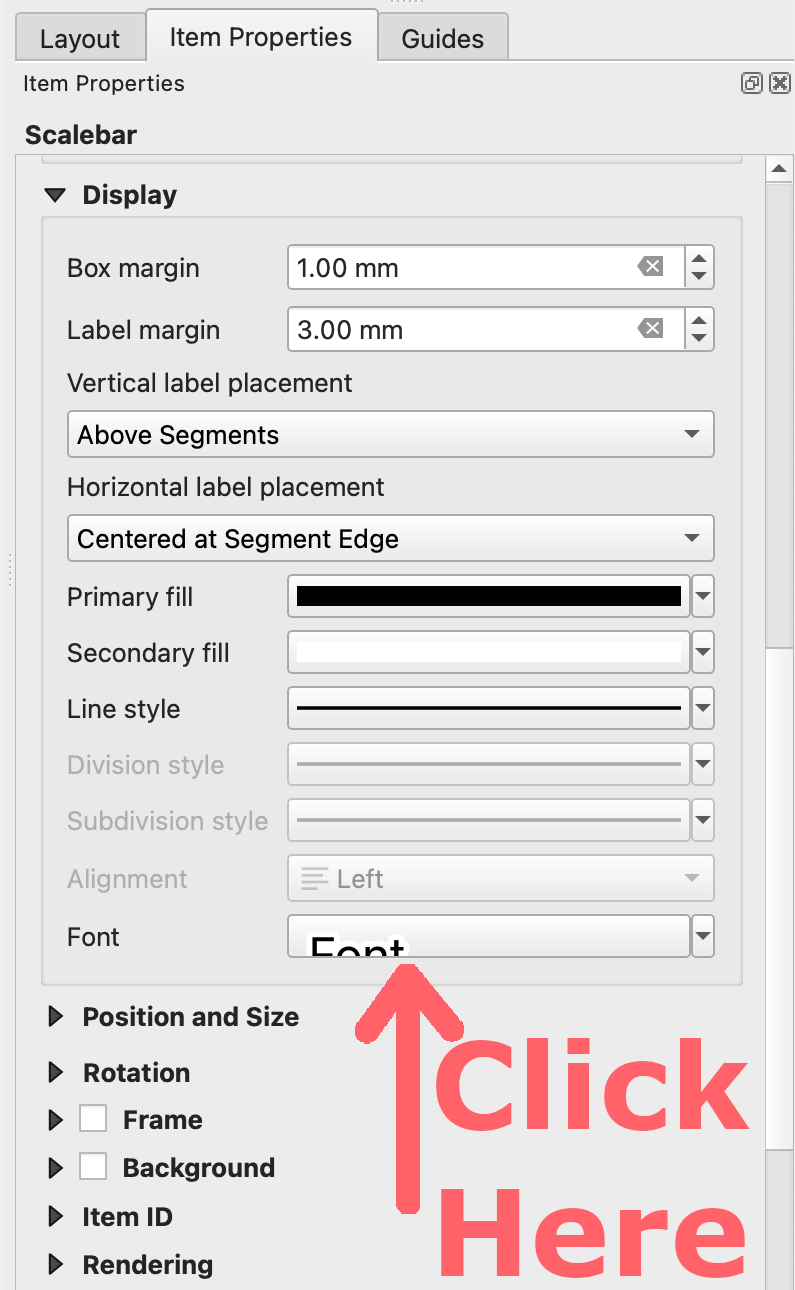
\includegraphics[width=.24\textwidth]{AdjustScalebar.png}}

Click on the highlighted text button and select the box that states ``Draw Text Buffer''. Adjust the size, color, and opacity as you see fit. We kept the defaults. 

\subsection{Adding a North Arrow}

On maps, it is also customary to use an arrow to indicate which direction is North. This is particularly useful again when zoomed in this closely, and the reader is unable to make out discernible land marks like state/country borders, large lakes/rivers, or oceans/coastlines. 

\vspace{.25em}

\centerline{\includegraphics[width=\textwidth]{AddNorthArrow.png}}

21. Click the \textit{Add Item} menu at the top of the screen and select \textit{Add North Arrow}.

22. Select your preferred North arrow symbol. Draw the North arrow in an appropriate place; they are typically placed near the scalebar. We will use the SVG north arrow that looks like a compass, but keep it small and out of the way of the map.

\kulbox{\textbf{NOTE:} When adding images to your map, \textit{SVG Images} tend to look cleaner and sharper compared to the \textit{Raster Image} options because of the way they store information. Just as we talked about in \href{https://jeremydforsythe.github.io/icecream-tutorials/Tutorial3_DrawingAreaOfInterest/Tutorial3_DrawingAreaOfInterest.pdf}{Tutorial \#3 : Drawing An Area of Interest} for raster vs vector GIS data, raster images are built from pixels - tiny color squares that, in great quantity, can form highly detailed images such as photographs. The more pixels an image has, the higher quality it will be, and vice versa. Vector files use mathematical equations, lines, and curves with fixed points on a grid to produce an image. There are no pixels in a vector file. A vector file’s mathematical formulas capture shape, border, and fill color to build an image. Because the mathematical formula recalibrates to any size, you can scale a vector image up or down without impacting its quality, which is why they tend to look cleaner and more professional.}

23. To adjust the properties of the North arrow to make it your own, scroll down in the \textit{Item Properties} window to find useful features, such as changing color or size. 

\subsection{Adding a Title}

\centerline{\includegraphics[width=\textwidth]{AddTitle.png}}

One last addition, let's add a title to the map to better orient the reader to the map's main message. 

24. Click the \textit{Add Item} menu at the top of the screen and select \textit{Add Label}.

25. Click on your map and draw a box where you want the title to be located. 

26. On the Item Properties tab, expand the Label section, and enter the text to title the map. For example, you could write ``Death Valley Extreme Surface Temperatures''.

27. You may want to change the spacing to make it look clean and professional. By clicking inside the \textit{Appearance} dropdown box, you can change the font size, text, color, backgrounds, etc. You can also adjust the alignment. For example, you could set it to \textit{Center} horizontal alignment and \textit{Middle} vertical.

28. To change the font options select the ABC tab, to change the background click the tab that looks like a highway sign. For further direction, see the screenshot on the next page.

29.  We chose the font ``Rockwell'' in size 30 white, with a red opaque ellipse background. We adjusted the Size Y to 3 millimeters to fully surround the text. You could copy these choices (see screenshot on the next page), but we encourage you to play around with these settings to make the map your own. Keep in mind the map making principles that we are discussing in class. It might also be a good idea to look at a \href{https://science.nasa.gov/earth/multimedia/}{gallery of NASA maps} or \href{https://mapgallery.esri.com/}{award winning maps from the ESRI Map Gallery} for inspiration. 

\centerline{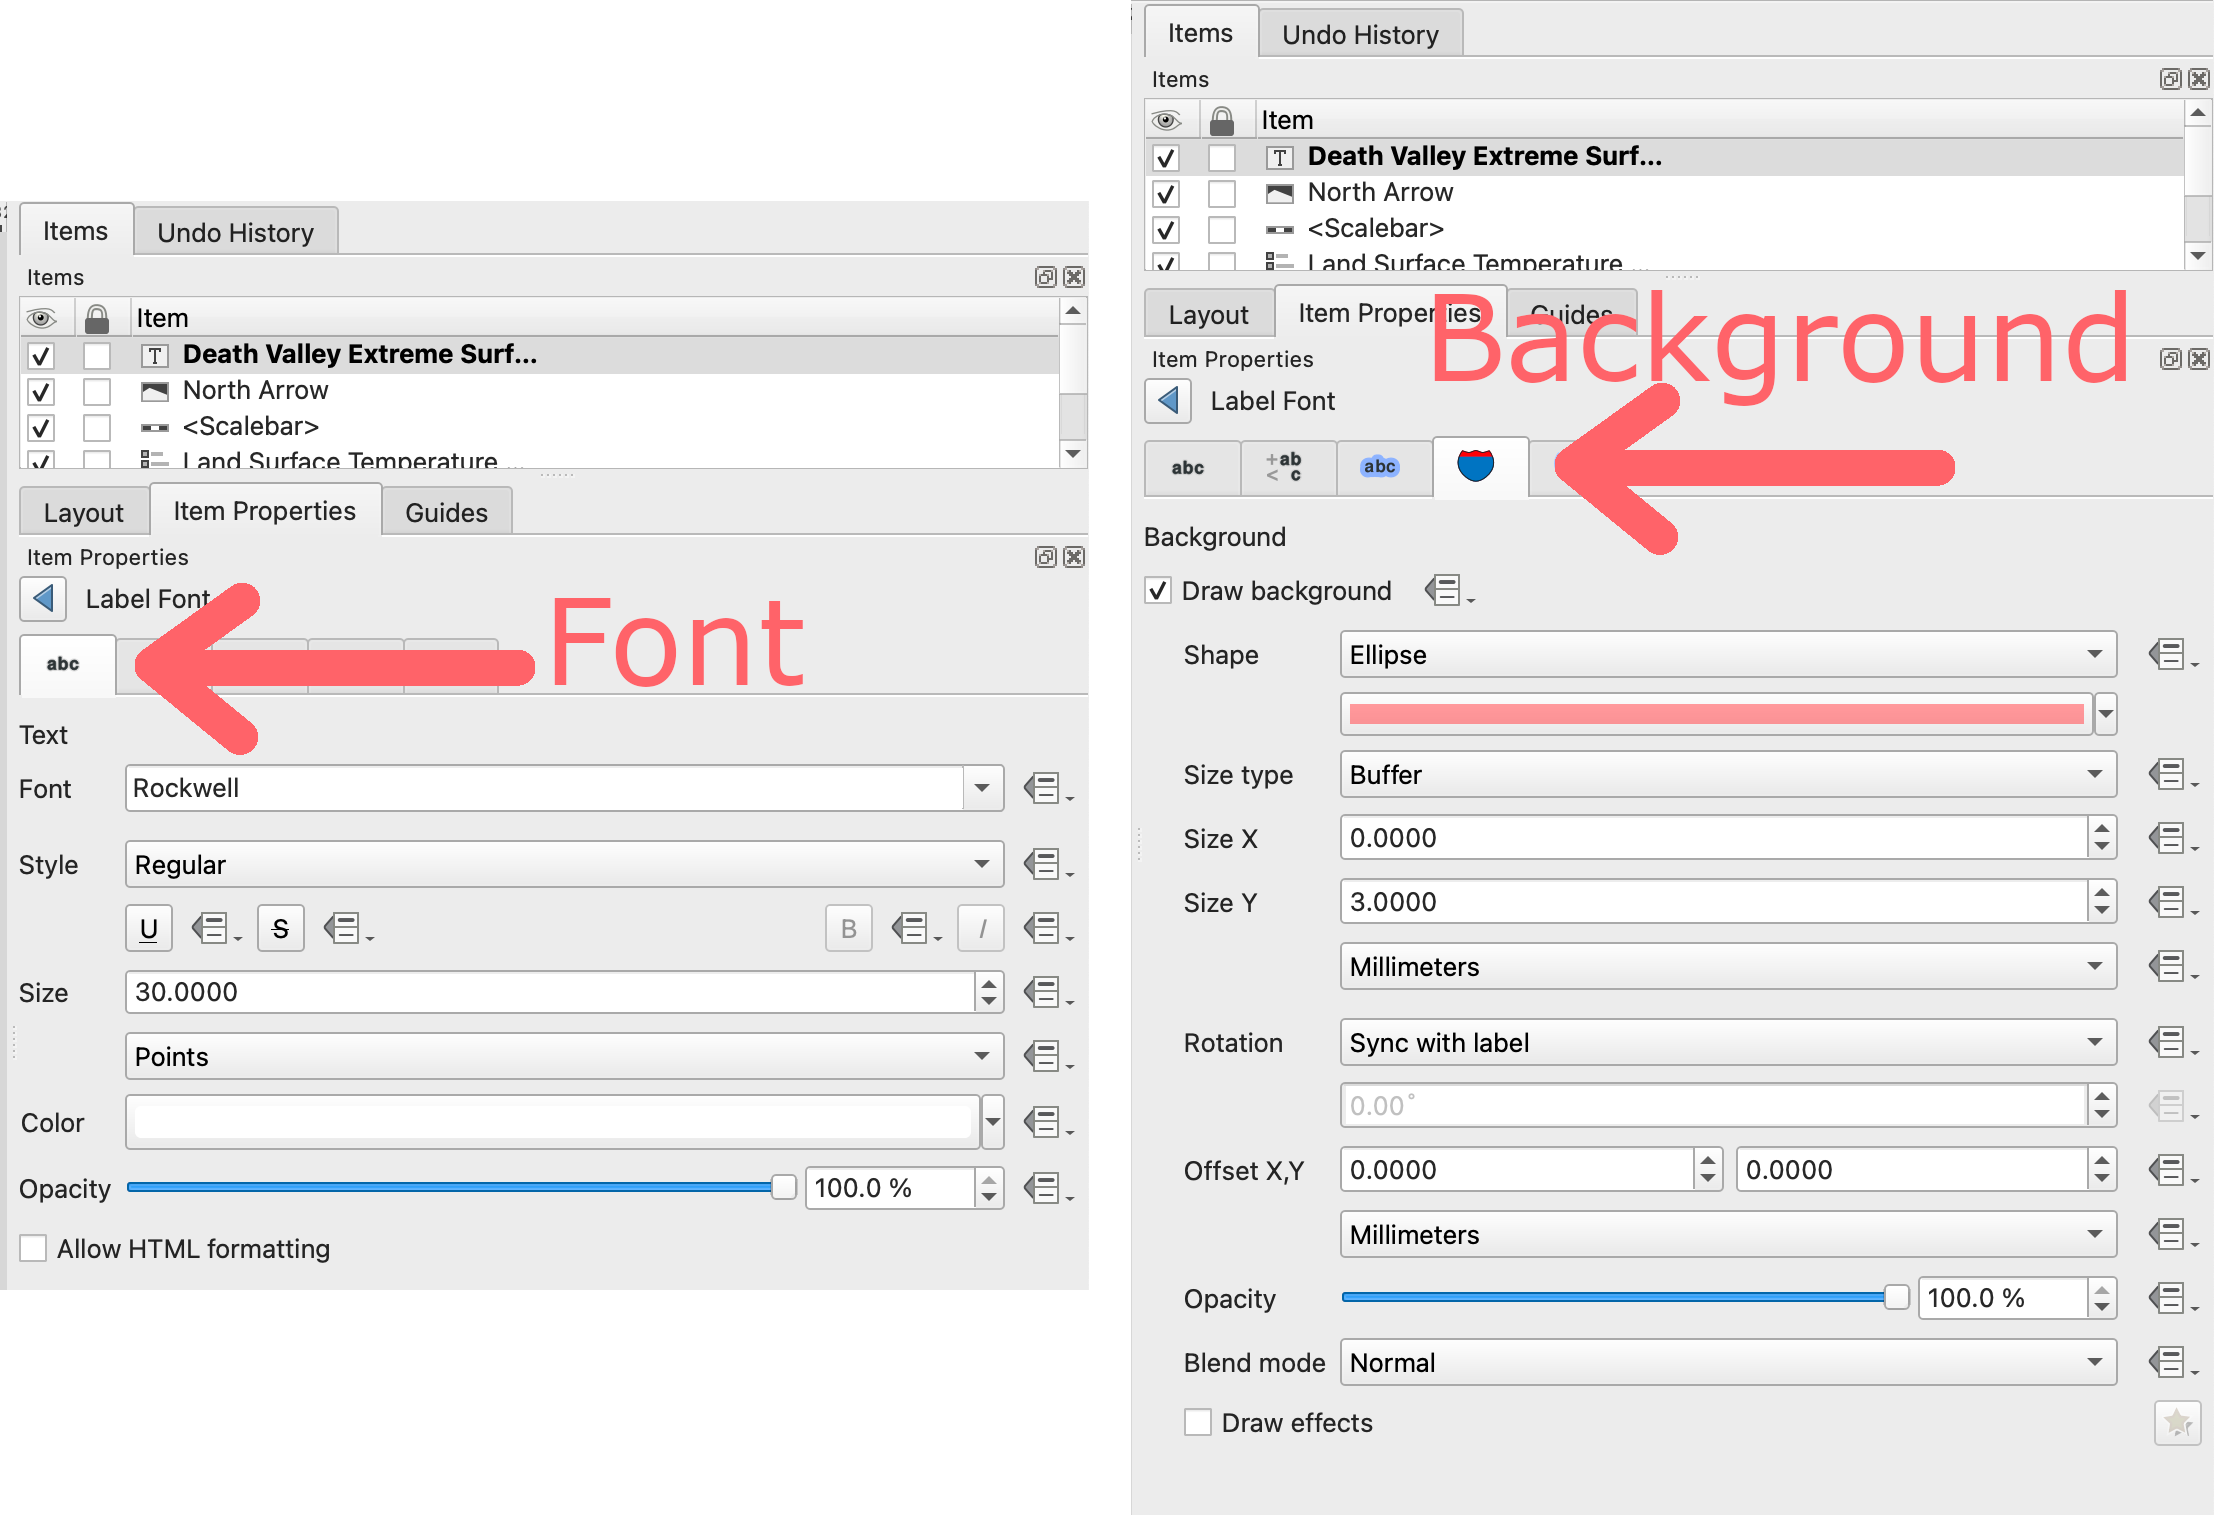
\includegraphics[width=.75\textwidth]{AdjustTitle.png}}

\section{Exporting Your Map}

\centerline{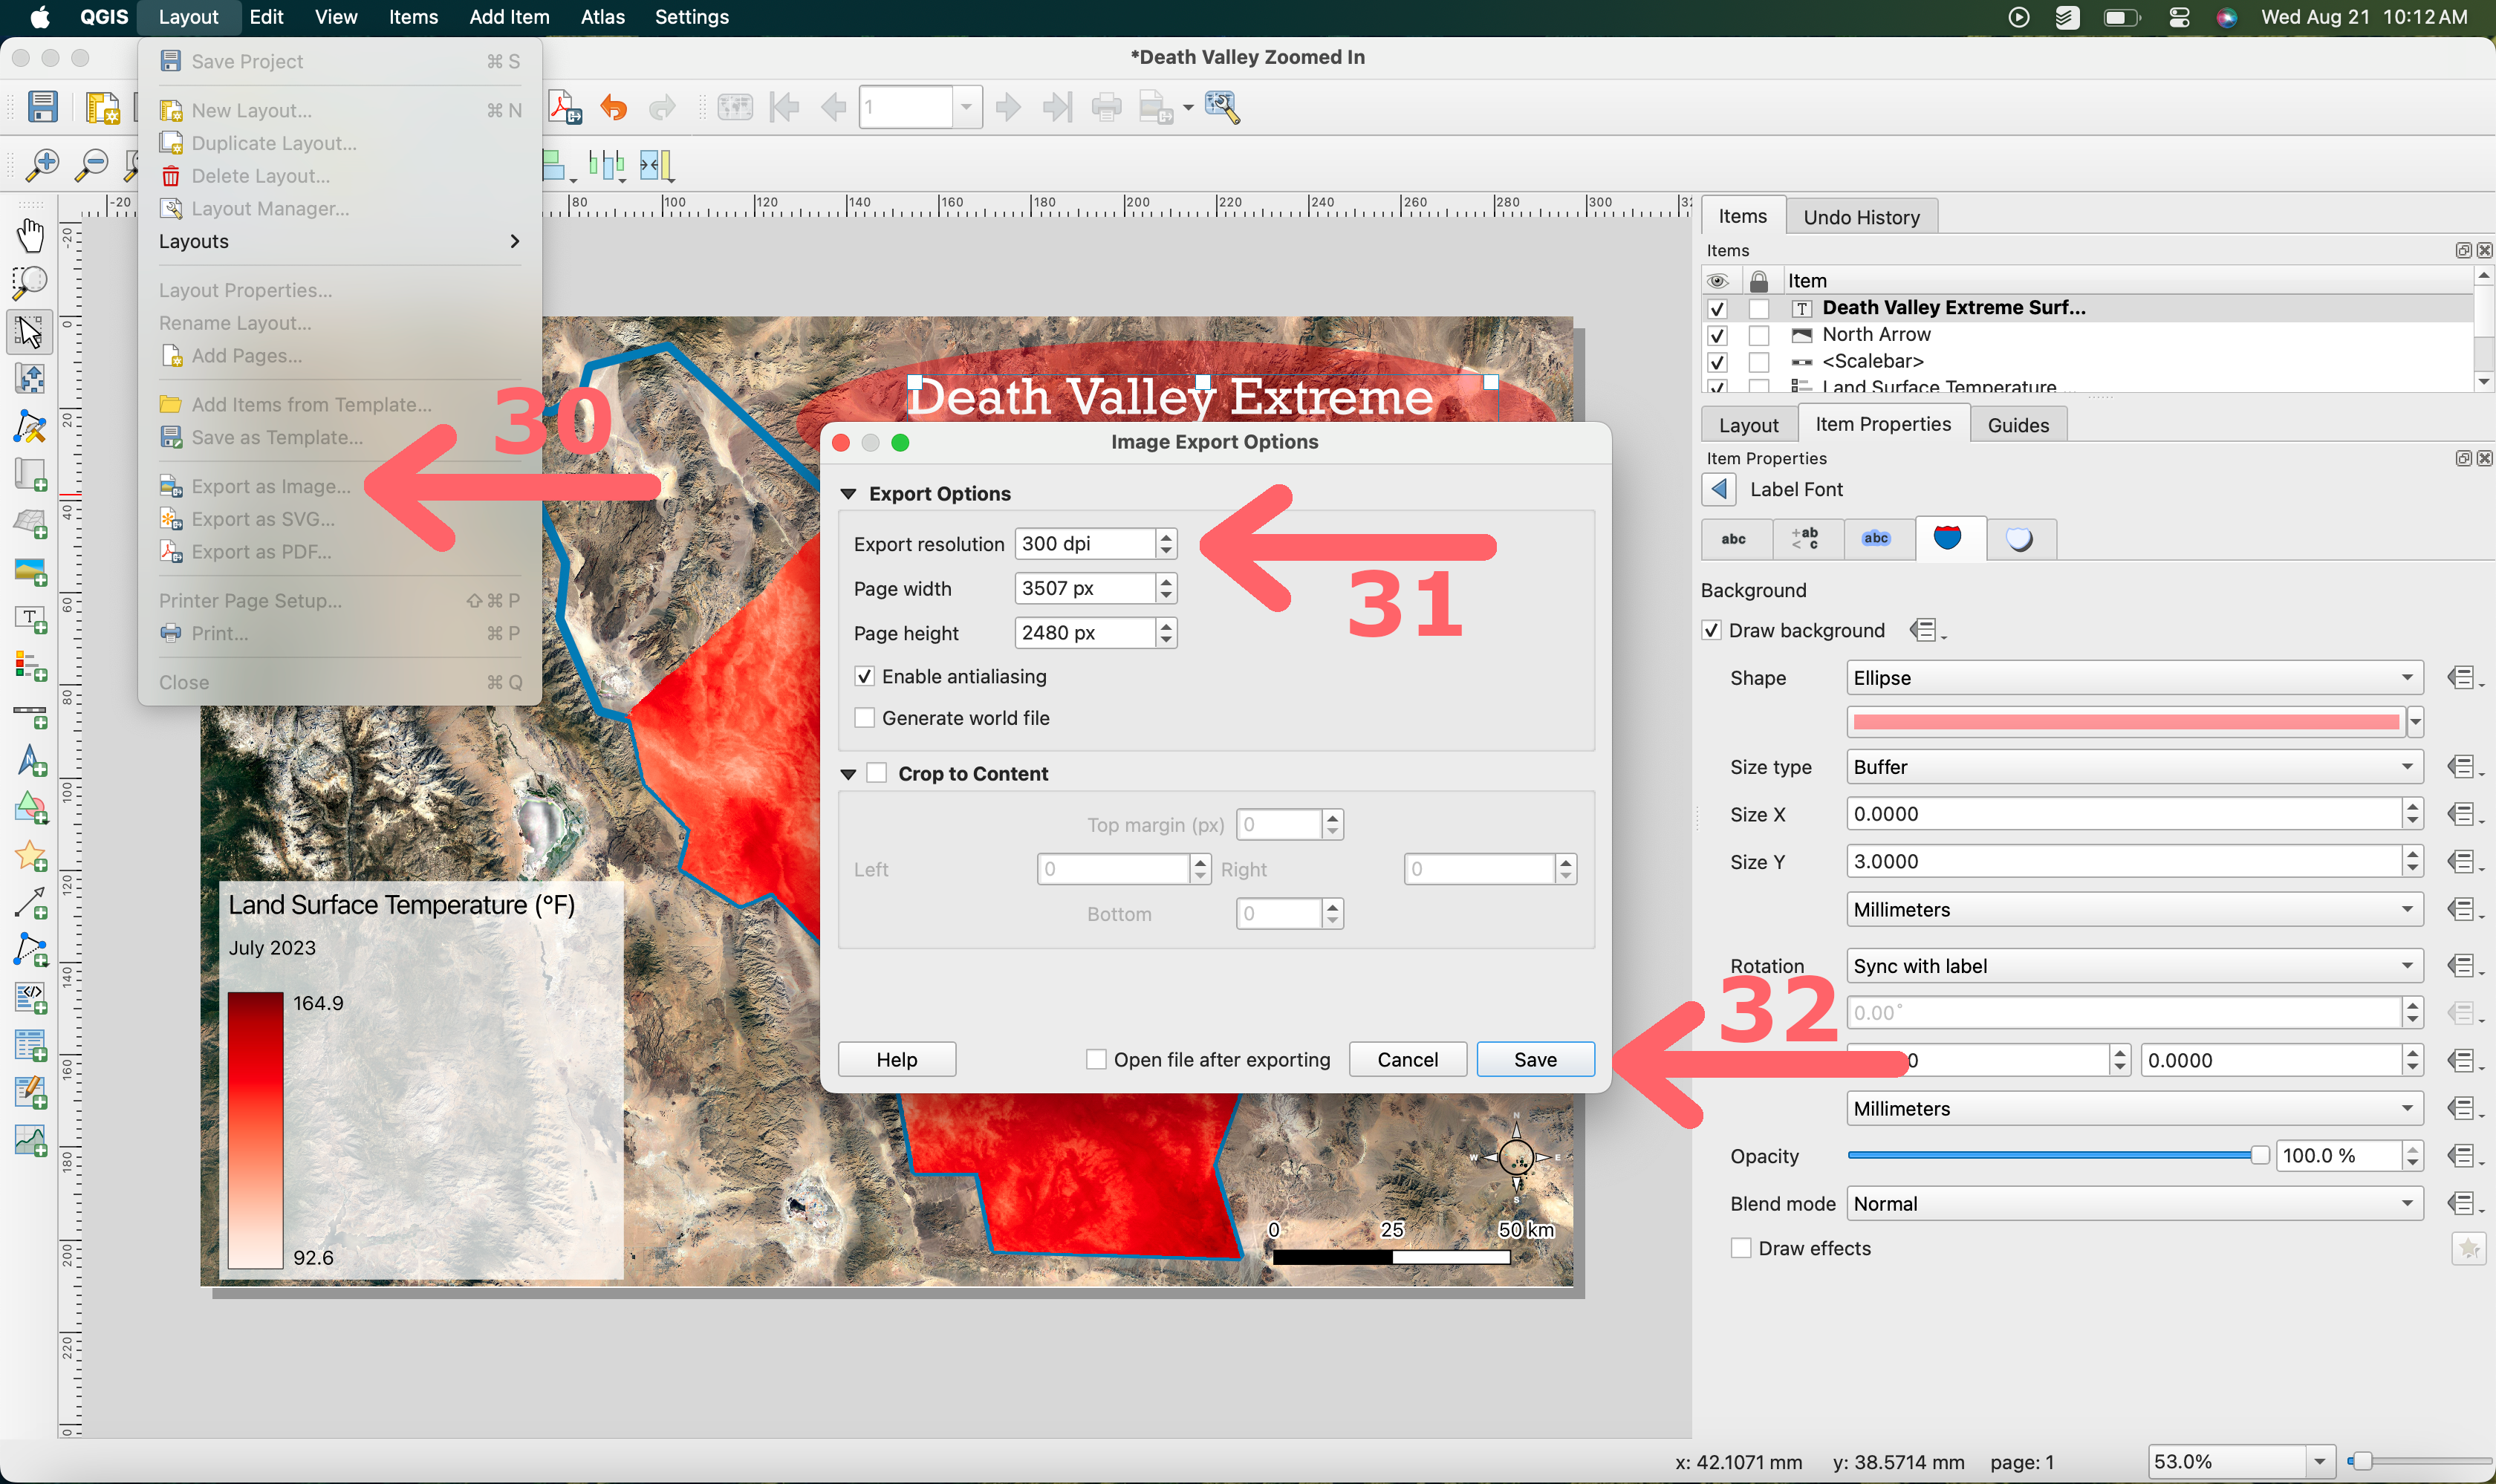
\includegraphics[width=\textwidth]{MapExport.png}}

Now that our map looks exactly how we want it to look, we want to be able to share it.

30. Select the \textit{Layout} dropdown menu, then \textit{Export as Image}. 

31. The \textit{Export resolution} controls how much detail the output image contains. Smaller resolution $=$ smaller file size, but with less detail. More resolution $=$ more detail saved, but larger file size. If storage is an issue for you, go with 100 dpi. Otherwise, 300 dpi will generally capture the detail in most cases.

32. Click \textit{Save} and bask in the glory of your first ECOSTRESS map. Congratulations...you did a thing!

\kulbox{\textbf{NOTE:} There may be times when you want to export as PDF, particularly when the map needs to be scalable to different sizes.}

Here is our final map for reference: 

\centerline{\includegraphics[width=.75\textwidth]{DeathValleyFinalMap.png}}

\section{Answering Our Original Question}

\centerline{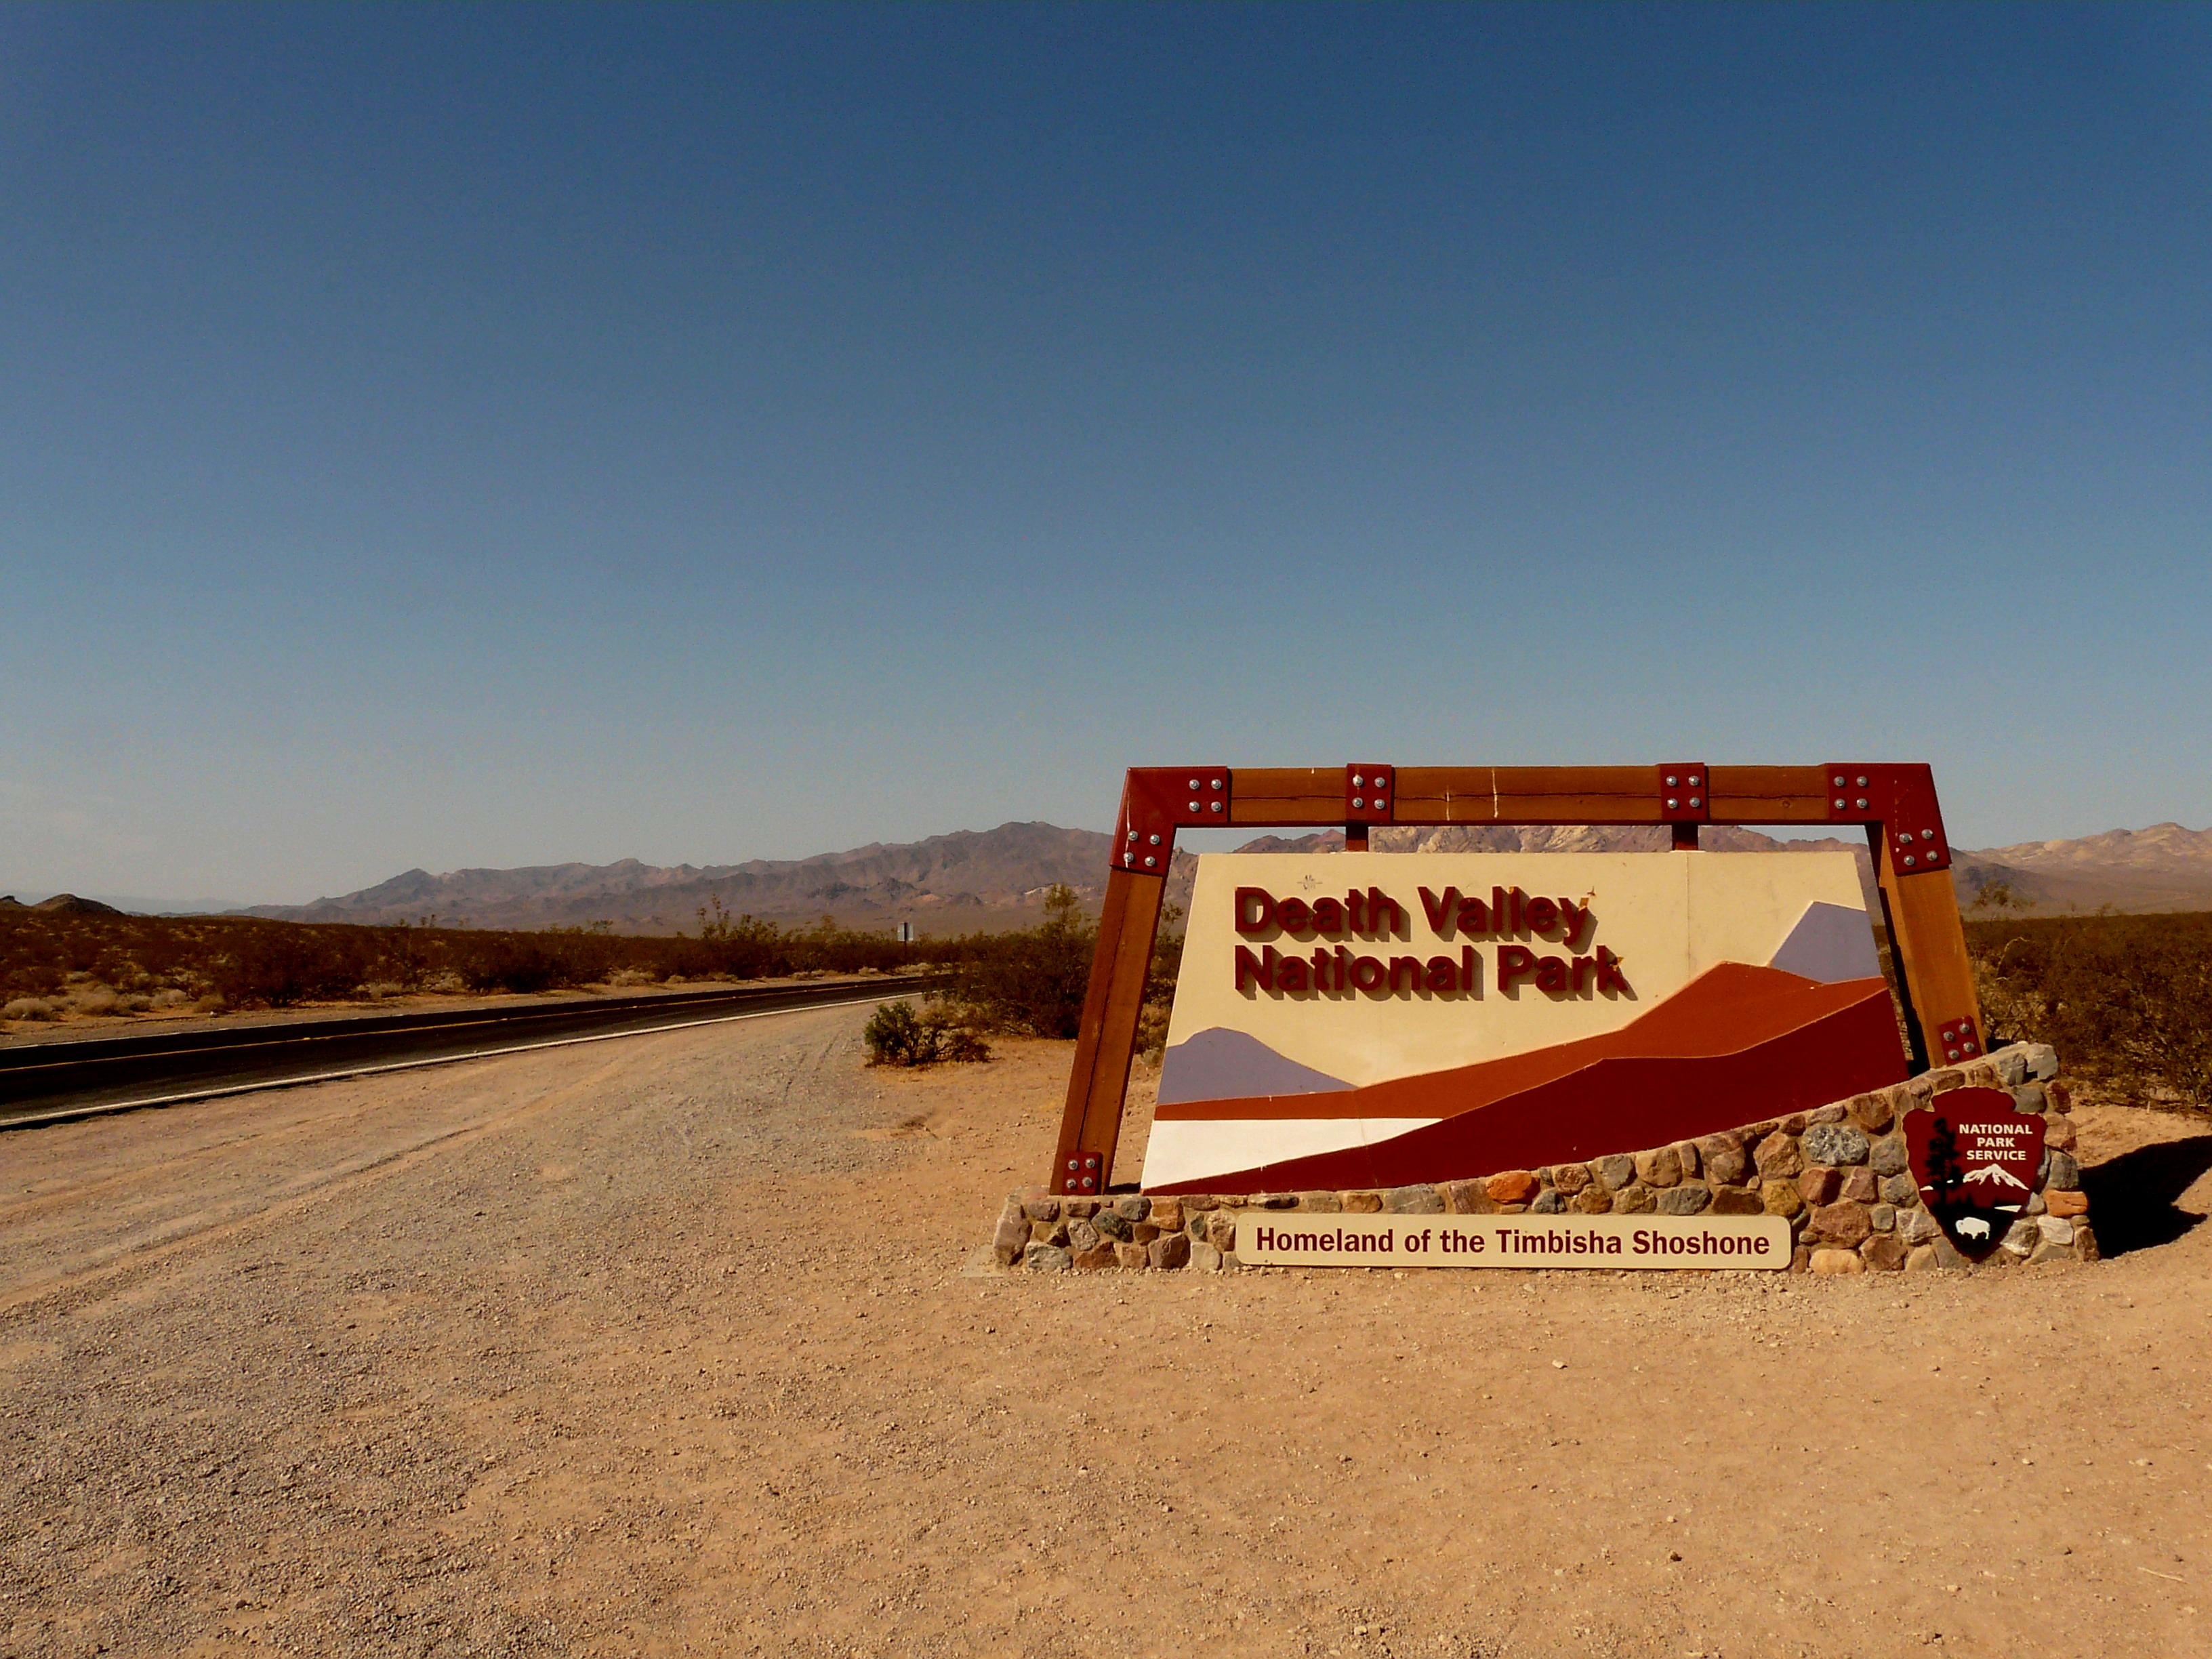
\includegraphics[width=.675\textwidth]{DeathValleySign.jpg}}

Our motivation for this exercise was to see if an analysis with ECOSTRESS supported our hypothesis that land surface temperatures in Death Valley National Park were close to breaking the surface temperature record. The highest recorded ground temperature of 201 $^{\circ}$F was verified on July 15, 1972. Does our analysis support that the record was broken in July 2023, given that it was one of the hottest months in recorded history for air temperatures?

\kulbox{\textbf{NOTE:} It is important to remember that the process of science ``supports'' or ``does not support'' hypotheses. It does not ``prove'' or ``disprove'' ideas. There are many factors that prevent our analyses from being entirely conclusive. These include the measurement error of our instruments, the times of day the International Space Station passed over the study site, cloudiness, etc.}

The real power of the ECOSTRESS satellite lies in its geographic and temporal continuity. For example, it is easy to see from our map which parts of Death Valley have the highest surface temperature. We could also track this seasonally to see how vegetation growth alters temperatures. The possibilities are endless.

\vspace{1em}

\begin{tcolorbox}[colback=yellow!5!white,colframe=MACred,title= \vspace{.2em} \Large Make a Map Assignments]
    \addcontentsline{toc}{section}{Make a Map Assignments}
    \large
    \begin{enumerate}
        \item Watch the YouTube Video: \href{https://www.youtube.com/watch?v=K24kSpOGssE}{Careers in Observing Earth from Above - Fernando Emiliano Romero Galvan}
        \item Build two hometown maps, one with the hottest temperature observed and a second with the coldest temperature observed. Put the maps on an appropriate baselayer with the outline of your polygon. 
        \item Find a classmate and compare maps. Is your classmate doing anything differently that can help improve your maps? If so, revise accordingly! 
        \item Submit your land surface temperature maps, along with a short description. In particular, your description might address any interesting observations about the temperature and address any limitations of your analysis.
    \end{enumerate}
\end{tcolorbox}

%%%%%%%%%%%%%%%%%%%%%%%%%%%%%%%%%%%%%%%%%%%%%%%%%%%%%%%%%%%%%%%%%%%%%%%%%%%%%%%%%%% End of Document
\vfill

\hrule

\vspace{1em}

\small \textbf{Recommended Citation:} Forsythe, J.D., G.R. Goldsmith, and J.B. Fisher. 2023. Observing Earth from Above Tutorials. Chapman University. \url{https://jeremydforsythe.github.io/icecream-tutorials/}

\vspace{1em}

This work is supported by funding from NASA ECOSTRESS Mission Grant \#80NSSC23K0309 (I.C.E. C.R.E.A.M.: Integrating Communication of ECOSTRESS Into Community Research, Education, Applications, and Media) and is openly licensed via \href{https://creativecommons.org/licenses/by-nc/4.0/}{CC BY-NC}.

\end{document}
